% Dokumentklassen s�ttes til memoir.
% Manual: http://ctan.org/tex-archive/macros/latex/contrib/memoir/memman.pdf
\documentclass[a4paper,oneside,article]{memoir}

\usepackage{pgf}
\usepackage{tikz}
\usepackage{pgfplots}
\usetikzlibrary{arrows,automata}
\usepackage{verbatim}
 
% Danske udtryk (fx figur og tabel) samt dansk orddeling og fonte med
% danske tegn. Hvis LaTeX brokker sig over �, � og � skal du udskifte
% "utf8" med "latin1" eller "applemac". 
\usepackage{inputenc}
\usepackage[danish]{babel}
\usepackage[T1]{fontenc}
 
% Matematisk udtryk, fede symboler, theoremer og fancy ting (fx k�debr�ker)
\usepackage{amsmath,amssymb}
\usepackage{bm}
\usepackage{amsthm}
%\usepackage{mathtools}
 
% Kodelisting. Husk at l�se manualen hvis du vil lave fancy ting.
% Manual: http://mirror.ctan.org/macros/latex/contrib/listings/listings.pdf
\usepackage{listings}
 
% Fancy ting med enheder og datatabeller. L�s manualen til pakken
% Manual: http://www.ctan.org/tex-archive/macros/latex/contrib/siunitx/siunitx.pdf
%\usepackage{siunitx}

% Inds�ttelse af grafik.
\usepackage{graphicx}
\usepackage{float}
\usepackage{caption}
\usepackage{subcaption}
 
% Reaktionsskemaer. L�s manualen for at se eksempler.
% Manual: http://www.ctan.org/tex-archive/macros/latex/contrib/mhchem/mhchem.pdf
%\usepackage[version=3]{mhchem}
%\usepackage[noend]{algpseudocode}
%\usepackage{algorithm}

\usepackage{xcolor,colortbl}

\usepackage{listings}

\definecolor{javared}{rgb}{0.6,0,0} % for strings
\definecolor{javagreen}{rgb}{0.25,0.5,0.35} % comments
\definecolor{javapurple}{rgb}{0.5,0,0.35} % keywords
\definecolor{javadocblue}{rgb}{0.25,0.35,0.75} % javadoc

\lstset{language=Java,
basicstyle=\small, %\ttfamily,
keywordstyle=\color{javapurple}\bfseries,
stringstyle=\color{javared},
commentstyle=\color{javagreen},
morecomment=[s][\color{javadocblue}]{/**}{*/},
numbers=left,
numberstyle=\tiny\color{black},
stepnumber=1,
numbersep=10pt,
tabsize=4,
showspaces=false,
showstringspaces=false}

\newcommand{\notimplies}{%
  \mathrel{{\ooalign{\hidewidth$\not\phantom{=}$\hidewidth\cr$\implies$}}}}

\begin{document}
    \title{Logical Clocks - Disposition}
    \author{Lukas Peter J�rgensen, 201206057, DA4
            }
    \maketitle
        
    \chapter{The happens-before relation}
    When you just need a well-defined ordering of events and not physical time. For example an online-forum, where we want all answers to be posted after the questions and we want all answers to be in the same order on all replicas of the forum.\\
    That is, all we care about is whether event A \textit{happened before} event B.
    \begin{figure}[H]
    	\centering
        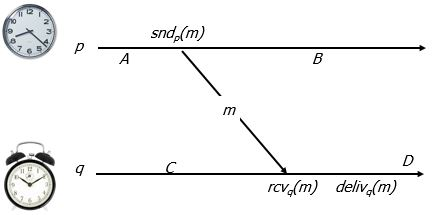
\includegraphics{Media/Time-Line.jpg}
    \end{figure}
    
    \subsection*{Local ordering}
    A happens before $snd_p(m)$ which happens before B, and C before $rcv_q(m)$ which happens before D.\\
    This is the local ordering, at each individual process, denoted:
    $$A\overset{p}{\rightarrow}snd_p(m)\overset{p}{\rightarrow}B$$
    And
    $$C\overset{q}{\rightarrow}rcv_q(m)\overset{q}{\rightarrow}D$$
    
    \subsection*{Distributed ordering}
    $snd_p(m)$ happens before $rcv_q(m)$, this is the distributed ordering of the system, denoted:
    $$snd_p(m)\overset{M}{\rightarrow}rcv_q(m)$$
    
    \subsection*{Transitive ordering}
    Since $A\rightarrow snd_p(m)$ and $snd_p\rightarrow rcv_q(m)$ we get that $A\rightarrow rcv_q(m)$ and therefore $A\rightarrow D$.
    
    \subsection*{Concurrent ordering}
    $B$ and $D$ are \textit{concurrent}, even though it looks like B happens before D, there is know way of knowing since no information have flowed between the two processes.
    
    \section{Lamport's logical clocks}
    Each process holds a local counter $C_p$ (integer) and everytime an event that matters to $p$ happens at a process $p$, the process increments $C_p$.\\
    When $p$ sends $m$ it sets:
    $$C_m=C_p$$
    When $q$ receives $m$ set:
    $$C_q=max(C_q,C_m)+1$$
    
    From previous image:
    $$C(A)=1, C(snd_p(m))=2,C(m)=2,C(B)=3$$
    $$C(C)=1,C(rcv_q(m))=max(1,2)+1=3,C(deliver_q(m))=4,C(D)=5$$
    \subsection*{Comparison with Happens-Before}
    If $A\overset{p}{\rightarrow} B$ then $C(A)<C(B)$\\
    If $A\overset{M}{\rightarrow}B$ then $C(B)=C(A)+1$\\
    If not $A\overset{p}{\rightarrow}B$ or $A\overset{M}{\rightarrow}B$, and there exist C such that $A\rightarrow C\rightarrow B;$ induction says $C(A)<C(C)$ and $C(C)<C(B)$, so $C(A)<C(B)$.\\
    \\
    \textbf{But,} $C(A)<C(B)\notimplies A\rightarrow B$.\\
    \textbf{Because,} processes that don't communicate still assign timestamps and hence events will "seem" to have an order.\\
    For example:
    \begin{figure}[H]
    \centering
    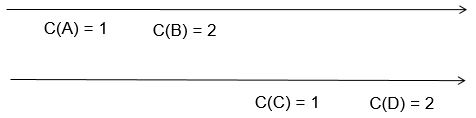
\includegraphics{Media/clockvshappensbefore.jpg}
    \end{figure}
    So $C(C)<C(B)$ but we don't have $C\rightarrow B$.
    
    \chapter{Totally Ordered Multicasting}
	In som situations we'd want an additional requirement, that no two events ever occur at exactly the same time. To achieve this goal, we can attach the ID of the process in which the event occurs to the low-order end of the time i.e. after the decimal point. For example an event at time $40$ at process $P_i$ will be timestamped $40.i$.\\
    With this additional requirement, Lamport's logical clocks can be used to implement totally-ordered multicasts.\\
    $P_1$ writes 'a' at time 1, $P_2$ writes 'b' at time 1, both add them to a local queue: $Q(P_1) = \{('a',1.1)\}$, $Q(P_2) = \{'b'.1.2\}$\\
    $P_1$ recieves 'b' which is timestamped $1.2$ and $P_2$ recieves 'a' which is timestamped $1.1$ both insert them into the queue:\\
    $Q(P_1) = \{('a',1.1),('b',1.2)\},$ $Q(P_2) = \{('a',1.1),('b',1.2)\}$\\
    They now end up with same copies of the queues, they will now send out acknowledgements for the recieved messages and they can then be sent to the application.
    
    \chapter{Vector clocks}
    Can capture causality.
    
    Let each process $P_i$ maintain a vector $VC_i$ with the following two properties:\\
    $VC_i[i]$ is the number of events that have occured so far at $P_i$ in other words, $VC_i[i]$ is the local logical clock at process $P_i$.
    If $VC_i[j]=k$, then $P_i$ knows that k events have occured at $P_j$. It is thus $P_i$'S knowledge of the local time at $P_j$\\
    \\
    The two properties are maintained by following the three following rules, similar to lamport clocks:\\
    When event happens at $p$, increment $VC_p[index_p]$.\\
    When sending a message, set $VC(M)=VC_p$.\\
    When receiving, set $VC_q=max(VC_q,VC(M))$ where max is max on each component of the vector.\\ 
    \\
    We now know how many events at other processes have taken place before $P_i$ sent message $m$, we can now make enforce causal ordering by delaying any recieved message recieved by $P_j$ from $P_i$ with timestamp $ts(m)$ until the following two conditions are met:
    $$1.\text{ }ts(m)[i]=VC_j[i]+1$$
    $$2.\text{ }ts(m)[k]\leq VC_j[k]\text{ for all } k \neq i$$
    1. states that $m$ is the next message that $P_j$ was expecting from process $P_i$, the second condition states that $P_j$ has seen all the messages that have been seen by $P_i$.
    
\end{document}